\section*{Problem Statement}
The thesis will focus on parliamentary proceedings from the German
\emph{Bundestag}. These proceedings are available online as PDF files dating
back to 1949, and have used essentially the same document layout and conventions
since the start. These PDF files can be converted to an XML representation which
retains much of the PDF makeup, or to unstructured plaintext which only
preserves newlines. Figure~\ref{fig:example} shows an excerpt from an arbitrary
source PDF file, along with the two possible representations.

\begin{figure}[htbp]
  \centering
  \begin{subfigure}[b]{0.4\textwidth} 
    \centering
    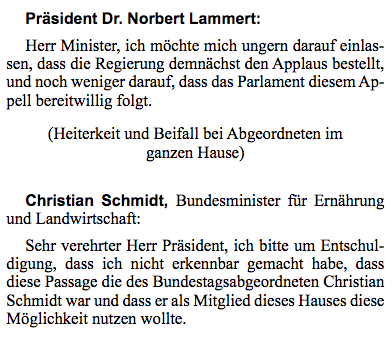
\includegraphics[width=\textwidth]{figures/source.png}
    \caption{The source PDF}
  \end{subfigure}
  \begin{subfigure}[b]{0.59\textwidth}
	\centering
    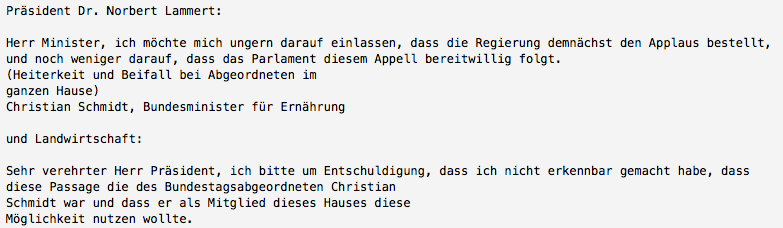
\includegraphics[width=\textwidth]{figures/plain.png}
    \caption{Plaintext}
    \vspace{2ex}
    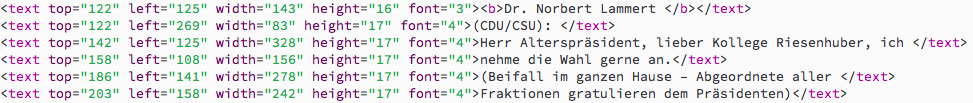
\includegraphics[width=\textwidth]{figures/xml.png}
    \caption{XML}
  \end{subfigure}
  \caption{The different data representations}
  \label{fig:example}
\end{figure}

The documents are composed of a sequence of topics, each topic having a title
and containing a series of speeches. Each of these speeches has a speaker, who
in turn have either a party or a role (e.g.\ minister or president). The task is
to parse this information, or as much of it as feasible, from the documents. The
start of each document features a table of contents, outlining the topics and
the speeches within them by page number. For some reason, speeches by the
president are excluded from this table of contents.

The dataset, obtained through a rule-based system as described in the
introduction, is currently complete dating back to 2005. It features 811
documents, containing 143.446 speeches spread over 7877 topics. This range can
be extended further back into the past to obtain more data, but the further back
the less reliable the data becomes.
